\begin{pastexam}[label={px:ntu-115-bmei-alg-03}]{臺大生醫電資所 115 學年度 第 3 題}
（問答）

(6\%) Please draw the binary search tree after successively inserting keys 8, 3, 1, 4, 9, 6, 7, 2, 5
into an initially empty tree.
\end{pastexam}

\begin{pastsoln}
每次插入都從根往下比：比目前節點小往左、大往右，走到空的位置就放下去（資結書第~9.2~節）。
\begin{center}
\small
\begin{tabular}{cll}
\toprule
插入 & 比較路徑 & 放在 \\
\midrule
8 & （空樹） & 根 \\
3 & $3 < 8$ & 8 的左子節點 \\
1 & $1 < 8$，$1 < 3$ & 3 的左子節點 \\
4 & $4 < 8$，$4 > 3$ & 3 的右子節點 \\
9 & $9 > 8$ & 8 的右子節點 \\
6 & $6 < 8$，$6 > 3$，$6 > 4$ & 4 的右子節點 \\
7 & $7 < 8$，$7 > 3$，$7 > 4$，$7 > 6$ & 6 的右子節點 \\
2 & $2 < 8$，$2 < 3$，$2 > 1$ & 1 的右子節點 \\
5 & $5 < 8$，$5 > 3$，$5 > 4$，$5 < 6$ & 6 的左子節點 \\
\bottomrule
\end{tabular}
\end{center}
最後的樹：
\begin{center}
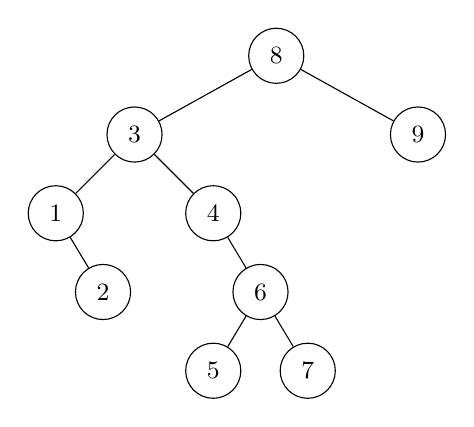
\begin{tikzpicture}[level distance=10mm,
  every node/.style={circle,draw,minimum size=7mm,inner sep=0pt,font=\small},
  level 1/.style={sibling distance=36mm}, level 2/.style={sibling distance=20mm},
  level 3/.style={sibling distance=12mm}]
\node {8}
  child {node {3}
    child {node {1} child[missing] child {node {2}}}
    child {node {4} child[missing] child {node {6} child {node {5}} child {node {7}}}}}
  child {node {9}};
\end{tikzpicture}
\end{center}
檢查：中序走訪是 $1, 2, 3, 4, 5, 6, 7, 8, 9$，遞增，是 BST（資結書定理~9.1）。 樹高 $5$ 層（$8 \to 3 \to
4 \to 6 \to 5$ 或 $7$），前序是 $8, 3, 1, 2, 4, 6, 5, 7, 9$。 畫圖時要畫出左右：$2$ 是 $1$ 的\textbf{右}子節點，
$6$ 是 $4$ 的\textbf{右}子節點，只有一個子節點時不能畫在正下方。
\end{pastsoln}
